\documentclass[12pt]{article}
\usepackage{amsmath,amssymb}
\usepackage[margin=1in]{geometry}
\usepackage{array}
\usepackage{tikz}
\usetikzlibrary{arrows.meta,calc}
\setlength{\parindent}{0pt}
\setlength{\parskip}{4pt}

\begin{document}

\noindent
\textbf{Name: Sindayen, Lorenzo Danilo V.}

\noindent
\textbf{APM1220 - Applied Multivariate Data Analysis}

\vspace{0.4cm}
\hrule
\vspace{0.5cm}

\textbf{INSTRUCTIONS:}

\begin{itemize}
    \item Answer all questions completely and show all necessary steps, intermediate calculations, and mathematical proofs clearly to receive full credit.
    \item Where matrix operations are required, ensure that dimensions conform before performing any multiplications, additions, or inversions.
    \item Present all final matrix entries and numerical results in exact, simplified form (e.g., fractions or radicals) unless decimals are specifically requested.
    \item Clearly label your final answers for each sub-problem (a, b, c, etc.).
\end{itemize}

\vspace{0.3cm}
\hrule
\vspace{0.7cm}

\section*{Problem 3.1}

\vspace{0.2cm}

Given the data matrix

\vspace{0.2cm}

\[
X=\begin{bmatrix}
9&1\\
5&3\\
1&2
\end{bmatrix}
\]

\vspace{0.2cm}

The three observations are $(9,1)$, $(5,3)$, and $(1,2)$

\vspace{0.2cm}

\subsection*{(a) Graph the scatter plot in $p=2$ dimensions. Locate the sample mean on your diagram.}

\vspace{0.2cm}

\textbf{Sol.}

\vspace{0.2cm}

The sample mean of each variable is

\vspace{0.2cm}

\[
\bar{x}_1=\frac{9+5+1}{3}=5,
\qquad
\bar{x}_2=\frac{1+3+2}{3}=2
\]

\vspace{0.2cm}

Thus,

\vspace{0.2cm}

\[
\boxed{\bar{\boldsymbol{x}}=(5,2)}
\]

\vspace{0.2cm}

The scatter plot below shows the observations and the sample mean.

\vspace{0.2cm}

\begin{center}
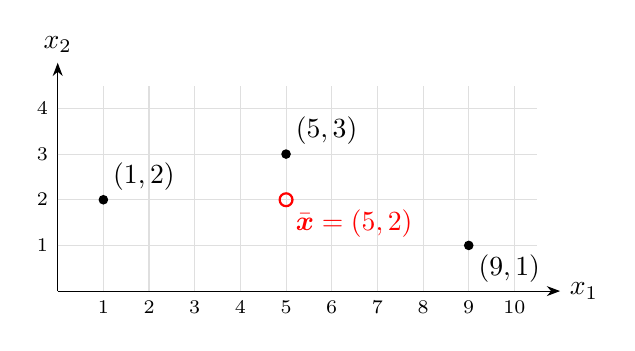
\begin{tikzpicture}[scale=0.58,>=Stealth]
  \draw[->] (0,0)--(11,0) node[right] {$x_1$};
  \draw[->] (0,0)--(0,5) node[above] {$x_2$};
  \foreach \x in {1,...,10} \draw[gray!25] (\x,0)--(\x,4.5);
  \foreach \y in {1,...,4} \draw[gray!25] (0,\y)--(10.5,\y);
  \foreach \x in {1,...,10} \node[below] at (\x,0) {\scriptsize \x};
  \foreach \y in {1,...,4} \node[left] at (0,\y) {\scriptsize \y};
  \fill (9,1) circle (3pt) node[below right] {$(9,1)$};
  \fill (5,3) circle (3pt) node[above right] {$(5,3)$};
  \fill (1,2) circle (3pt) node[above right] {$(1,2)$};
  \draw[red,thick] (5,2) circle (4pt);
  \node[red,below right] at (5,2) {$\bar{\boldsymbol{x}}=(5,2)$};
\end{tikzpicture}
\end{center}

\vspace{0.2cm}

\subsection*{(b) Sketch the $n=3$-dimensional representation of the data, and plot the deviation vectors
$\boldsymbol{y}_1-\bar{x}_1\boldsymbol{1}$ and
$\boldsymbol{y}_2-\bar{x}_2\boldsymbol{1}$.}

\vspace{0.2cm}

\textbf{Sol.}

\vspace{0.2cm}

Writing each variable as a vector in $\mathbb{R}^3$ gives

\vspace{0.2cm}

\[
\boldsymbol{y}_1=\begin{bmatrix}9\\5\\1\end{bmatrix},
\qquad
\boldsymbol{y}_2=\begin{bmatrix}1\\3\\2\end{bmatrix},
\qquad
\boldsymbol{1}=\begin{bmatrix}1\\1\\1\end{bmatrix}
\]

\vspace{0.2cm}

Therefore, the deviation vectors are

\vspace{0.2cm}

\[
\boldsymbol{y}_1-\bar{x}_1\boldsymbol{1}
=\begin{bmatrix}9\\5\\1\end{bmatrix}
-5\begin{bmatrix}1\\1\\1\end{bmatrix}
=\boxed{\begin{bmatrix}4\\0\\-4\end{bmatrix}},
\]
and
\[
\boldsymbol{y}_2-\bar{x}_2\boldsymbol{1}
=\begin{bmatrix}1\\3\\2\end{bmatrix}
-2\begin{bmatrix}1\\1\\1\end{bmatrix}
=\boxed{\begin{bmatrix}-1\\1\\0\end{bmatrix}}
\]

\vspace{0.2cm}

Both deviation vectors lie in the plane perpendicular to $\boldsymbol{1}$, because their components each sum to zero. The following schematic represents the centered vectors in three-dimensional observation space.

\vspace{0.2cm}

\begin{center}
\begin{tikzpicture}[scale=0.75,>=Stealth]
  \draw[->] (0,0)--(4.5,0) node[right] {$e_1$};
  \draw[->] (0,0)--(1.6,2.7) node[above] {$e_2$};
  \draw[->] (0,0)--(-1.5,-2.3) node[below left] {$e_3$};
  \draw[->,blue,very thick] (0,0)--(3.2,0.1) node[above right] {$\boldsymbol{y}_1-\bar{x}_1\boldsymbol{1}$};
  \draw[->,red,very thick] (0,0)--(-0.7,1.4) node[above left] {$\boldsymbol{y}_2-\bar{x}_2\boldsymbol{1}$};
  \fill (0,0) circle (2pt) node[below right] {$O$};
\end{tikzpicture}
\end{center}

\vspace{0.2cm}

The sketch is schematic; the exact coordinates of the vectors are the three-component vectors calculated above.

\vspace{0.2cm}

\subsection*{(c) Sketch the deviation vectors in (b) emanating from the origin. Calculate their lengths and the cosine of the angle between them. Relate these quantities to $S_n$ and $R$.}

\vspace{0.2cm}

\textbf{Sol.}

\vspace{0.2cm}

Let
\[
\boldsymbol{d}_1=\begin{bmatrix}4\\0\\-4\end{bmatrix},
\qquad
\boldsymbol{d}_2=\begin{bmatrix}-1\\1\\0\end{bmatrix}
\]

\vspace{0.2cm}

Their lengths are

\vspace{0.2cm}

\[
\|\boldsymbol{d}_1\|
=\sqrt{4^2+0^2+(-4)^2}
=\sqrt{32}
=\boxed{4\sqrt{2}},
\]

\vspace{0.2cm}

\[
\|\boldsymbol{d}_2\|
=\sqrt{(-1)^2+1^2+0^2}
=\sqrt{2}
=\boxed{\sqrt{2}}
\]

\vspace{0.2cm}

The dot product is

\vspace{0.2cm}

\[
\boldsymbol{d}_1'\boldsymbol{d}_2
=4(-1)+0(1)+(-4)(0)=-4
\]

\vspace{0.2cm}

Hence, the cosine of the angle $\theta$ between them is

\vspace{0.2cm}

\[
\cos\theta
=\frac{\boldsymbol{d}_1'\boldsymbol{d}_2}
{\|\boldsymbol{d}_1\|\|\boldsymbol{d}_2\|}
=\frac{-4}{(4\sqrt{2})(\sqrt{2})}
=\boxed{-\frac12}
\]

\vspace{0.2cm}

Using the centered data matrix $D=[\boldsymbol{d}_1\ \boldsymbol{d}_2]$,

\vspace{0.2cm}

\[
D' D=
\begin{bmatrix}
32&-4\\
-4&2
\end{bmatrix}
\]

\vspace{0.2cm}

With the $n$-divisor convention, $S_n=\frac1nD'D$, so

\vspace{0.2cm}

\[
\boxed{
S_n=\begin{bmatrix}
\frac{32}{3}&-\frac43\\
-\frac43&\frac23
\end{bmatrix}}
\]

\vspace{0.2cm}

The diagonal entries are the coordinate-wise mean squared deviations; equivalently, the squared lengths satisfy $\|\boldsymbol{d}_j\|^2=n(S_n)_{jj}$. The off-diagonal entry records the inner product divided by $n$. The correlation matrix is

\vspace{0.2cm}

\[
R=\begin{bmatrix}
1&\dfrac{-4}{\sqrt{32}\sqrt{2}}\\
\dfrac{-4}{\sqrt{32}\sqrt{2}}&1
\end{bmatrix}
=\boxed{\begin{bmatrix}1&-\frac12\\-\frac12&1\end{bmatrix}}
\]

\vspace{0.2cm}

Thus, the cosine between the centered data vectors equals the correlation between the two variables. If sample covariance is defined with divisor $n-1$, then
$S=\frac12D'D=\begin{bmatrix}16&-2\\-2&1\end{bmatrix}$; its correlation matrix is the same $R$.

\vspace{0.7cm}
\hrule
\vspace{0.7cm}

\section*{Problem 3.6}

\vspace{0.2cm}

Consider the data matrix

\vspace{0.2cm}

\[
X=\begin{bmatrix}
-1&3&-2\\
2&4&2\\
5&2&3
\end{bmatrix}
\]

\vspace{0.2cm}

\subsection*{(a) Calculate the matrix of deviations (residuals), $X-\boldsymbol{1}\bar{\boldsymbol{x}}'$. Is this matrix of full rank? Explain.}

\vspace{0.2cm}

\textbf{Sol.}

\vspace{0.2cm}

The column means are

\vspace{0.2cm}

\[
\bar{x}_1=\frac{-1+2+5}{3}=2,\qquad
\bar{x}_2=\frac{3+4+2}{3}=3,\qquad
\bar{x}_3=\frac{-2+2+3}{3}=1
\]

\vspace{0.2cm}

Therefore,

\vspace{0.2cm}

\[
\bar{\boldsymbol{x}}'=\begin{bmatrix}2&3&1\end{bmatrix},
\qquad
\boldsymbol{1}\bar{\boldsymbol{x}}'
=\begin{bmatrix}
2&3&1\\
2&3&1\\
2&3&1
\end{bmatrix}\
\]

\vspace{0.2cm}

Subtracting gives

\vspace{0.2cm}

\[
X-\boldsymbol{1}\bar{\boldsymbol{x}}'
=\begin{bmatrix}
-1-2&3-3&-2-1\\
2-2&4-3&2-1\\
5-2&2-3&3-1
\end{bmatrix}
=\boxed{\begin{bmatrix}
-3&0&-3\\
0&1&1\\
3&-1&2
\end{bmatrix}}
\]

\vspace{0.2cm}

Each column of the residual matrix sums to zero, so its columns lie in the two-dimensional subspace perpendicular to $\boldsymbol{1}\in\mathbb{R}^3$. Consequently, its rank is at most $3-1=2$. The first two columns are not scalar multiples of each other, so the rank is exactly $2$. Therefore, the residual matrix is \textbf{not} of full rank $3$.

\vspace{0.2cm}

\subsection*{(b) Determine \(S\) and calculate the generalized sample variance \(|S|\). Interpret the latter geometrically.}

\vspace{0.2cm}

\textbf{Sol.}

\vspace{0.2cm}

For \(n=3\) observations, the sample covariance matrix is

\vspace{0.2cm}

\[
S=\frac{1}{n-1}
(X-\boldsymbol{1}\bar{\boldsymbol{x}}')
'(X-\boldsymbol{1}\bar{\boldsymbol{x}}')
=\frac12D'D
\]

\vspace{0.2cm}

Using the residual matrix \(D\) from part (a),

\vspace{0.2cm}

\[
D'D=
\begin{bmatrix}
18&-3&15\\
-3&2&-1\\
15&-1&14
\end{bmatrix}
\]

\vspace{0.2cm}

Thus,

\vspace{0.2cm}

\[
\boxed{
S=\begin{bmatrix}
9&-\frac32&\frac{15}{2}\\
-\frac32&1&-\frac12\\
\frac{15}{2}&-\frac12&7
\end{bmatrix}
}
\]

\vspace{0.2cm}

The generalized sample variance is the determinant of \(S\):

\vspace{0.2cm}

\[
|S|=
\begin{vmatrix}
9&-\frac32&\frac{15}{2}\\
-\frac32&1&-\frac12\\
\frac{15}{2}&-\frac12&7
\end{vmatrix}
=\boxed{0}
\]

\vspace{0.2cm}

Geometrically, the determinant of a covariance matrix measures the squared volume scale of the data ellipsoid (up to the relevant dimension-dependent constant). Since \(|S|=0\), the ellipsoid is degenerate and has zero three-dimensional volume. This is consistent with the centered data having rank \(2\), so the observations do not span all three variable dimensions after centering.

\vspace{0.2cm}

\subsection*{(c) Using the results in (b), calculate the total sample variance. [See (3-23).]}

\vspace{0.2cm}

\textbf{Sol.}

\vspace{0.2cm}

The total sample variance is the trace of the sample covariance matrix, that is, the sum of its diagonal entries:
\[
\operatorname{tr}(S)=s_{11}+s_{22}+s_{33}
=9+1+7.
\]
Therefore,
\[
\boxed{\text{Total sample variance}=17}
\]

\vspace{0.7cm}
\hrule
\vspace{0.7cm}

\section*{Problem 3.9}

The data matrix for the test scores is
\[
X=\begin{bmatrix}
12&17&29\\
18&20&38\\
14&16&30\\
20&18&38\\
16&19&35
\end{bmatrix},
\]
where $x_1$ and $x_2$ are the first and second test scores and $x_3$ is the total score.

\subsection*{(a) Obtain the mean-corrected data matrix, and verify that the columns are linearly dependent. Specify an $\boldsymbol{a}'=[a_1,a_2,a_3]$ vector that establishes the linear dependence.}

\vspace{0.2cm}

\textbf{Sol.}

\vspace{0.2cm}

The sample mean vector is

\vspace{0.2cm}

\[
\bar{\boldsymbol{x}}'
=\left[
\frac{12+18+14+20+16}{5},
\frac{17+20+16+18+19}{5},
\frac{29+38+30+38+35}{5}
\right]
=\begin{bmatrix}16&18&34\end{bmatrix}
\]

\vspace{0.2cm}

Subtracting the mean vector from each row gives

\vspace{0.2cm}

\[
D=X-\boldsymbol{1}\bar{\boldsymbol{x}}'
=\boxed{\begin{bmatrix}
-4&-1&-5\\
2&2&4\\
-2&-2&-4\\
4&0&4\\
0&1&1
\end{bmatrix}}
\]

\vspace{0.2cm}

The third column is the sum of the first and second columns:

\vspace{0.2cm}

\[
\boldsymbol{d}_3=\boldsymbol{d}_1+\boldsymbol{d}_2
\]

\vspace{0.2cm}

Equivalently,

\vspace{0.2cm}

\[
\boldsymbol{d}_1+\boldsymbol{d}_2-\boldsymbol{d}_3=\boldsymbol{0}.
\]

\vspace{0.2cm}

Thus the columns are linearly dependent. One vector establishing this dependence is

\vspace{0.2cm}

\[
\boxed{\boldsymbol{a}=\begin{bmatrix}1\\1\\-1\end{bmatrix},
\qquad
\boldsymbol{a}'=\begin{bmatrix}1&1&-1\end{bmatrix}}
\]

\vspace{0.2cm}

\subsection*{(b) Obtain the sample covariance matrix $S$, and verify that the generalized variance is zero. Also, show that $S\boldsymbol{a}=0$, so $\boldsymbol{a}$ can be rescaled to be an eigenvector corresponding to eigenvalue zero.}

\vspace{0.2cm}

\textbf{Sol.}

\vspace{0.2cm}

There are $n=5$ observations, so

\vspace{0.2cm}

\[
S=\frac{1}{n-1}D'D=\frac14D'D
\]

\vspace{0.2cm}

The cross-products are

\vspace{0.2cm}

\[
D'D=
\begin{bmatrix}
40&12&52\\
12&10&22\\
52&22&74
\end{bmatrix}
\]

\vspace{0.2cm}

Therefore,

\vspace{0.2cm}

\[
\boxed{
S=\begin{bmatrix}
10&3&13\\
3&\frac52&\frac{11}{2}\\
13&\frac{11}{2}&\frac{37}{2}
\end{bmatrix}.}
\]

\vspace{0.2cm}

Because the third column is the sum of the first two, the covariance matrix is singular. Directly,

\vspace{0.2cm}

\[
|S|=\boxed{0}
\]

\vspace{0.2cm}

To verify the required null-vector relation,

\vspace{0.2cm}

\[
S\boldsymbol{a}
=
\begin{bmatrix}
10&3&13\\
3&\frac52&\frac{11}{2}\\
13&\frac{11}{2}&\frac{37}{2}
\end{bmatrix}
\begin{bmatrix}1\\1\\-1\end{bmatrix}
=
\begin{bmatrix}
10+3-13\\
3+\frac52-\frac{11}{2}\\
13+\frac{11}{2}-\frac{37}{2}
\end{bmatrix}
=
\boxed{\begin{bmatrix}0\\0\\0\end{bmatrix}}
\]

\vspace{0.2cm}

Hence, $\boldsymbol{a}$ is an eigenvector associated with eigenvalue $0$. It may be normalized, if desired, to $\boldsymbol{a}/\sqrt{3}$, which is also an eigenvector for eigenvalue zero. The generalized variance is zero because the data have an exact linear dependence among the three variables.

\subsection*{(c) Verify that the third column of the data matrix is the sum of the first two columns. That is, show that there is linear dependence, with $a_1=1$, $a_2=1$, and $a_3=-1$.}

\vspace{0.2cm}

\textbf{Sol.}

\vspace{0.2cm}

Checking the rows of the original data matrix:

\vspace{0.2cm}

\[
12+17=29,\quad
18+20=38,\quad
14+16=30,
\]

\vspace{0.2cm}

\[
20+18=38,\quad
16+19=35.
\]

\vspace{0.2cm}

Thus, for every observation, $x_{i3}=x_{i1}+x_{i2}$. In vector form,

\vspace{0.2cm}

\[
\boldsymbol{x}_1+\boldsymbol{x}_2-\boldsymbol{x}_3=\boldsymbol{0}
\]

\vspace{0.2cm}

Therefore, the columns are linearly dependent with coefficients

\vspace{0.2cm}

\[
\boxed{a_1=1,\qquad a_2=1,\qquad a_3=-1.}
\]

\vspace{0.2cm}

\vspace{0.7cm}
\hrule
\vspace{0.7cm}

\section*{Problem 3.18}

\textbf{Energy consumption in 2001, by state, from the major sources}

The variables are defined as follows:
\begin{itemize}
    \item $X_1 =$ petroleum
    \item $X_2 =$ natural gas
    \item $X_3 =$ hydroelectric power
    \item $X_4 =$ nuclear electric power
\end{itemize}

Energy consumption is recorded in quadrillions ($10^{15}$) of BTUs. The resulting mean vector and covariance matrix are given below.

\paragraph{Given mean vector}
\[
\bar{\mathbf{x}} = \begin{bmatrix}
0.766 \\
0.508 \\
0.438 \\
0.161
\end{bmatrix}
\]

\paragraph{Given covariance matrix}
\[
\mathbf{S} = \begin{bmatrix}
0.856 & 0.635 & 0.173 & 0.096 \\
0.635 & 0.568 & 0.128 & 0.067 \\
0.173 & 0.127 & 0.171 & 0.039 \\
0.096 & 0.067 & 0.039 & 0.043
\end{bmatrix}
\]

\vspace{0.7cm}

\subsection*{(a) Using the summary statistics, determine the sample mean and variance of a state's total energy consumption for these major sources}

\vspace{0.2cm}

\textbf{Sol.}

\vspace{0.2cm}

Let the total energy consumption be

\vspace{0.2cm}

\[
T = X_1 + X_2 + X_3 + X_4
\]

\vspace{0.2cm}

The sample mean of the total is obtained by adding the means of the four energy sources:

\vspace{0.2cm}

\begin{align*}
\bar{T} &= \bar{X}_1 + \bar{X}_2 + \bar{X}_3 + \bar{X}_4 \\
&= 0.766 + 0.508 + 0.438 + 0.161 \\
&= \boxed{1.873}
\end{align*}

\vspace{0.2cm}

The sample variance of the total is calculated by adding all entries of the covariance matrix, including the covariances between the different sources:

\vspace{0.2cm}

\[
\text{Var}(T) = \mathbf{1}' \mathbf{S} \mathbf{1}
\]

\vspace{0.2cm}

Therefore,

\vspace{0.2cm}

\begin{align*}
\text{Var}(T) &= 0.856 + 0.635 + 0.173 + 0.096 \\
&\quad + 0.635 + 0.568 + 0.128 + 0.067 \\
&\quad + 0.173 + 0.127 + 0.171 + 0.039 \\
&\quad + 0.096 + 0.067 + 0.039 + 0.043 \\
&= \boxed{3.913}
\end{align*}

\vspace{0.2cm}

Thus, the sample mean of total energy consumption is \textbf{1.873}, and the variance calculated from the supplied matrix entries is \textbf{3.913}.

\vspace{0.7cm}

\subsection*{(b) Determine the sample mean and variance of the excess of petroleum consumption over natural gas consumption. Also find the sample covariance of this variable with the total variable in part (a)}

\vspace{0.2cm}

\textbf{Sol.}

\vspace{0.2cm}

Let the excess of petroleum consumption over natural gas consumption be

\vspace{0.2cm}

\[
E = X_1 - X_2
\]

\vspace{0.2cm}

Define the coefficient vector

\vspace{0.2cm}

\[
\mathbf{c} = \begin{bmatrix}
1 \\
-1 \\
0 \\
0
\end{bmatrix}
\]

\vspace{0.2cm}

Then

\vspace{0.2cm}

\[
E = \mathbf{c}'\mathbf{X}
\]

\vspace{0.2cm}

The sample mean of the excess is:


\begin{align*}
\bar{E} &= \bar{X}_1 - \bar{X}_2 \\
&= 0.766 - 0.508 \\
&= \boxed{0.258}
\end{align*}

\vspace{0.2cm}

The sample variance of the excess is:

\vspace{0.2cm}

\[
\text{Var}(E) = s_{11} + s_{22} - 2s_{12}
\]

\vspace{0.2cm}

Substituting the given covariance matrix entries,

\vspace{0.2cm}

\begin{align*}
\text{Var}(E) &= 0.856 + 0.568 - 2(0.635) \\
&= 0.856 + 0.568 - 1.270 \\
&= \boxed{0.154}
\end{align*}

\vspace{0.2cm}

Next, the sample covariance between the excess $E$ and the total $T$ is:

\vspace{0.2cm}

\[
\text{Cov}(E, T) = \text{Cov}(X_1 - X_2, T)
\]

\vspace{0.2cm}

Using the covariance matrix entries as printed,

\vspace{0.2cm}

\[
\text{Cov}(E, T) = (s_{11} + s_{12} + s_{13} + s_{14}) - (s_{21} + s_{22} + s_{23} + s_{24})
\]

\vspace{0.2cm}

Substituting the values,

\vspace{0.2cm}

\begin{align*}
\text{Cov}(E, T) &= (0.856 + 0.635 + 0.173 + 0.096) - (0.635 + 0.568 + 0.128 + 0.067) \\
&= 1.760 - 1.398 \\
&= \boxed{0.362}
\end{align*}

\vspace{0.2cm}

Therefore, the sample mean of the excess is \textbf{0.258}, its sample variance is \textbf{0.154}, and its sample covariance with total energy consumption is \textbf{0.362}, using the matrix entries exactly as printed.

\vspace{0.7cm}
\hrule
\vspace{0.7cm}

\section*{Problem 3.20}

In northern climates, roads must be cleared of snow quickly following a storm. One measure of storm severity is $x_1$, its duration in hours, while the effectiveness of snow removal can be quantified by $x_2$, the number of hours crews, men, and machine spend to clear snow. Here are the results for 25 incidents in Wisconsin.

\subsection*{Table 3.2 Snow Data}

\begin{table}[h!]
\centering
\begin{tabular}{cccccc}
\toprule
$x_1$ & $x_2$ & $x_1$ & $x_2$ & $x_1$ & $x_2$ \\
\midrule
12.5 & 13.7 & 9.0  & 24.4 & 3.5  & 26.1 \\
14.5 & 16.5 & 6.5  & 18.2 & 8.0  & 14.5 \\
8.0  & 17.4 & 10.5 & 22.0 & 17.5 & 42.3 \\
9.0  & 11.0 & 10.0 & 32.5 & 10.5 & 17.5 \\
19.5 & 23.6 & 4.5  & 18.7 & 12.0 & 21.8 \\
8.0  & 13.2 & 7.0  & 15.8 & 6.0  & 10.4 \\
9.0  & 32.1 & 8.5  & 15.6 & 13.0 & 25.6 \\
7.0  & 12.3 & 6.5  & 12.0 &      &      \\
7.0  & 11.8 & 8.0  & 12.8 &      &      \\
\bottomrule
\end{tabular}
\end{table}

\vspace{0.2cm}

\subsection*{(a) Find the sample mean and variance of the difference $x_2 - x_1$ by first obtaining the summary statistics}

\vspace{0.2cm}

\textbf{Sol.}

\vspace{0.2cm}

Let $D = X_2 - X_1$, where $X_1$ represents storm duration and $X_2$ represents the crew-hours used to clear snow.

\vspace{0.2cm}

There are $n = 25$ observations. From the given data, the summary statistics are:
\begin{align*}
n &= 25 \\
\sum x_1 &= 235.5 \\
\sum x_2 &= 481.8 \\
\sum x_1^2 &= 2557.75 \\
\sum x_2^2 &= 10778.98 \\
\sum x_1 x_2 &= 4861.90
\end{align*}

\vspace{0.2cm}

The sample means are:
\[
\bar{x}_1 = \frac{235.5}{25} = 9.42
\]
\[
\bar{x}_2 = \frac{481.8}{25} = 19.272
\]

\vspace{0.2cm}

The sample mean of the difference is:
\begin{align*}
\bar{D} &= \bar{x}_2 - \bar{x}_1 \\
&= 19.272 - 9.42 \\
&= \boxed{9.852}
\end{align*}

\vspace{0.2cm}

The sample variances and covariance are calculated using the formula:
\[
s_{ik} = \frac{\sum x_i x_k - \dfrac{(\sum x_i)(\sum x_k)}{n}}{n - 1}
\]

\vspace{0.2cm}

Substituting the summary statistics:
\begin{align*}
s_{11} &= \frac{2557.75 - \dfrac{(235.5)^2}{25}}{24} = \frac{16967}{1200} \approx 14.1391667 \\[1em]
s_{22} &= \frac{10778.98 - \dfrac{(481.8)^2}{25}}{24} = \frac{1867163}{30000} \approx 62.2387667 \\[1em]
s_{12} &= \frac{4861.90 - \dfrac{(235.5)(481.8)}{25}}{24} = \frac{20209}{1500} \approx 13.4726667
\end{align*}

\vspace{0.2cm}

Using the variance formula for a difference,
\[
s_D^2 = s_{22} + s_{11} - 2s_{12}
\]

\vspace{0.2cm}

we obtain:
\begin{align*}
s_D^2 &= 62.2387667 + 14.1391667 - 2(13.4726667) \\
&= \boxed{49.4326}
\end{align*}

\vspace{0.2cm}

Therefore, the sample mean of the difference is \textbf{9.852}, and its sample variance is \textbf{49.4326}.

\vspace{0.2cm}

\subsection*{(b) Obtain the mean and variance by first obtaining the individual values $x_{j2} - x_{j1}$, for $j = 1, 2, \dots, 25$, and then calculating the mean and variance. Compare these values with those obtained in part (a)}

\vspace{0.2cm}

\textbf{Sol.}

\vspace{0.2cm}

Calculate the difference for each of the 25 incidents:

\vspace{0.2cm}

\begin{align*}
D_j = \{ &1.2, 2.0, 9.4, 2.0, 4.1, \\
& 5.2, 23.1, 5.3, 4.8, 15.4, \\
& 11.7, 11.5, 22.5, 14.2, 8.8, \\
& 7.1, 5.5, 4.8, 22.6, 6.5, \\
& 24.8, 7.0, 9.8, 4.4, 12.6 \}
\end{align*}

\vspace{0.2cm}

Their sum and sum of squares are:
\[
\sum_{j=1}^{25} D_j = 246.3
\]
\[
\sum_{j=1}^{25} D_j^2 = 3612.93
\]

\vspace{0.2cm}

The sample mean is:

\vspace{0.2cm}

\begin{align*}
\bar{D} &= \frac{\sum D_j}{n} \\
&= \frac{246.3}{25} \\
&= \boxed{9.852}
\end{align*}

\vspace{0.2cm}

The sample variance is:

\vspace{0.2cm}

\begin{align*}
s_D^2 &= \frac{\sum D_j^2 - \dfrac{(\sum D_j)^2}{n}}{n - 1} \\
&= \frac{3612.93 - \dfrac{(246.3)^2}{25}}{24} \\
&= \boxed{49.4326}
\end{align*}

\vspace{0.2cm}

Comparing the results with part (a), both methods give the same sample mean and variance:

\vspace{0.2cm}

\[
\boxed{\bar{D} = 9.852, \quad s_D^2 = 49.4326}
\]

\vspace{0.2cm}

Therefore, calculating the individual differences produces the same results as using the summary statistics, confirming that the two methods agree.

\end{document}